\documentclass[%
    school=etsisi,%
    degree=61TI,%
]{upm-report}

\title{Práctica 1: Diseño de un centro de datos bare metal}
\author{Miguel Hermoso Mantecón, Alejandro Fernández de la Puebla y Adolfo}

\begin{document}


\chapter{Contexto}
\label{ch:contexto}




\chapter{Diseño de la Arquitectura}
\label{ch:diseño-arquitectura}

La arquitectura de la red juega un papel fundamental en el rendimiento y eficiencia del sistema interconectado. La elección de una topología adecuada impacta directamente en aspectos como la latencia, el ancho de banda y el costo de implementación. 

\section{Elección de Topología}
\label{sec:elección-topología}

Una de las topologías más empleadas en grandes centros de datos y sistemas de cómputo de alto rendimiento es Dragonfly, debido a su capacidad para escalar y mantener bajas las latencias, incluso cuando el número de nodos aumenta. En este capítulo se profundiza en las decisiones relacionadas con la implementación de la arquitectura Dragonfly, discutiendo tanto su variante canónica como no canónica, así como la gestión de los grupos dentro de esta.

\section{Forma Canónica y no Canónica}
\label{sec:dragonfly}

Una vez seleccionada la topología Dragonfly para la red, es crucial definir qué tipo de configuración será la más adecuada: la Canónica o la No Canónica. Ambas variantes ofrecen diferentes niveles de complejidad y flexibilidad en la interconexión de nodos y grupos.

La Dragonfly \textit{Canónica} se caracteriza por una relación estricta entre el número de integrantes de un grupo y la cantidad de grupos en la red. En este caso, si se tienen $n$ nodos por grupo, habrá $n+1$ grupos en total. Esto garantiza que cada nodo esté conectado, como mínimo, a un grupo distinto, lo que optimiza la distribución del tráfico y facilita la gestión del enrutamiento. Esta relación predeterminada simplifica la planificación de la red y reduce la posibilidad de congestión, ya que se asegura una interconexión eficiente entre los grupos.

Por otro lado, la Dragonfly \textit{No Canónica} permite mayor flexibilidad al no imponer una relación fija entre la cantidad de nodos por grupo y el número de grupos. Esto podría ser útil en sistemas donde la heterogeneidad de los grupos es necesaria o donde se desea una mayor libertad a la hora de distribuir los recursos. Sin embargo, esta flexibilidad puede aumentar la complejidad de la configuración y la gestión, especialmente en redes de gran tamaño, ya que se pierden las ventajas de la regularidad que ofrece la versión canónica.

Se ha decidido implementar la Dragonfly Canónica en este diseño debido a su simplicidad y eficiencia en términos de costos. Al tener una estructura más regular y predecible, esta variante facilita la implementación del cableado, la gestión de direcciones IP y MAC, y el control del tráfico, todo lo cual es esencial para cumplir con los requisitos de la red.

\section{Gestión de los Grupos}
\label{sec:gestion-grupos}

Una vez definida la topología Dragonfly Canónica, es necesario determinar tanto el número de nodos por grupo como la cantidad total de grupos en la red. Para este caso, al trabajar con un total de 240 racks, se opta por una división en 15 nodos por grupo y 16 grupos. Esta configuración cumple con la restricción de tener n nodos por grupo y n+1 grupos, lo que asegura que la estructura de la red siga las características propias de la topología seleccionada.

El siguiente paso es establecer cómo se conectarán los diferentes grupos entre sí. Para optimizar el costo del cableado, se ha decidido que entre cada par de grupos solo existirá una conexión. Esto significa que dos grupos cualesquiera estarán unidos por un único enlace, resultando en un total de 15 enlaces externos por grupo. Cada nodo dentro de un grupo se identifica mediante un índice único, lo cual facilita la gestión de direcciones IP y MAC.

Para implementar las conexiones entre los grupos, se ha diseñado una estrategia de cableado basada en la correspondencia entre el índice del nodo y el grupo de destino. Es decir, cada nodo en un grupo estará conectado al nodo con el mismo índice en el grupo de destino. Por ejemplo, el nodo con ID 1 en el grupo 0 estará conectado al nodo con ID 0 en el grupo 1. No obstante, hay una excepción: un grupo no puede conectarse a sí mismo, por lo que no existirán enlaces internos dentro de un mismo grupo. Esto genera una situación particular en la que, debido a la topología Dragonfly Canónica, hay 1 grupo más que nodos por grupo. Esto significa que existe un grupo que no va a tener nodo con ID igual al grupo. Como resultado, este "grupo extra" se conectará a los demás grupos de la manera habitual, pero los demás grupos deberán utilizar el nodo con ID igual al grupo donde se encuentran para conectarse a este "grupo extra". Este comportamiento está ilustrado en la Figura X, donde se puede observar cómo se distribuyen los enlaces entre los nodos y grupos de la red, garantizando que cada nodo esté interconectado eficientemente dentro de la estructura Dragonfly.

\section{Conexiones con Internet}
\label{sec:conexiones-internet}

Para poder acatar el tráfico exterior, es necesario tener un router con conexión a Internet. Al contar con la topología Dragonfly de tipo Canónica, no queda más remedio que hacer que un nodo del grupo tenga tanto conexión a otro grupo como a Internet. Si bien es verdad que se podría haber gestionado de manera más intuitiva teniendo un nodo extra por grupo encargado de gestionar ese tráfico externo (ver la figura \ref{fig:no-canonica-internet}), el ratio eficiencia-recursos no es lo suficientemente grande como para decantarse por la Dragonfly No Canónica. Por ello, se ha decidido elegir al nodo con índice 0 de cada grupo como encargado de gestionar las conexiones al exterior (ver la figura \ref{fig:canonica-internet}).

\begin{figure}
    \centering
    \begin{subfigure}{0.49\textwidth}
        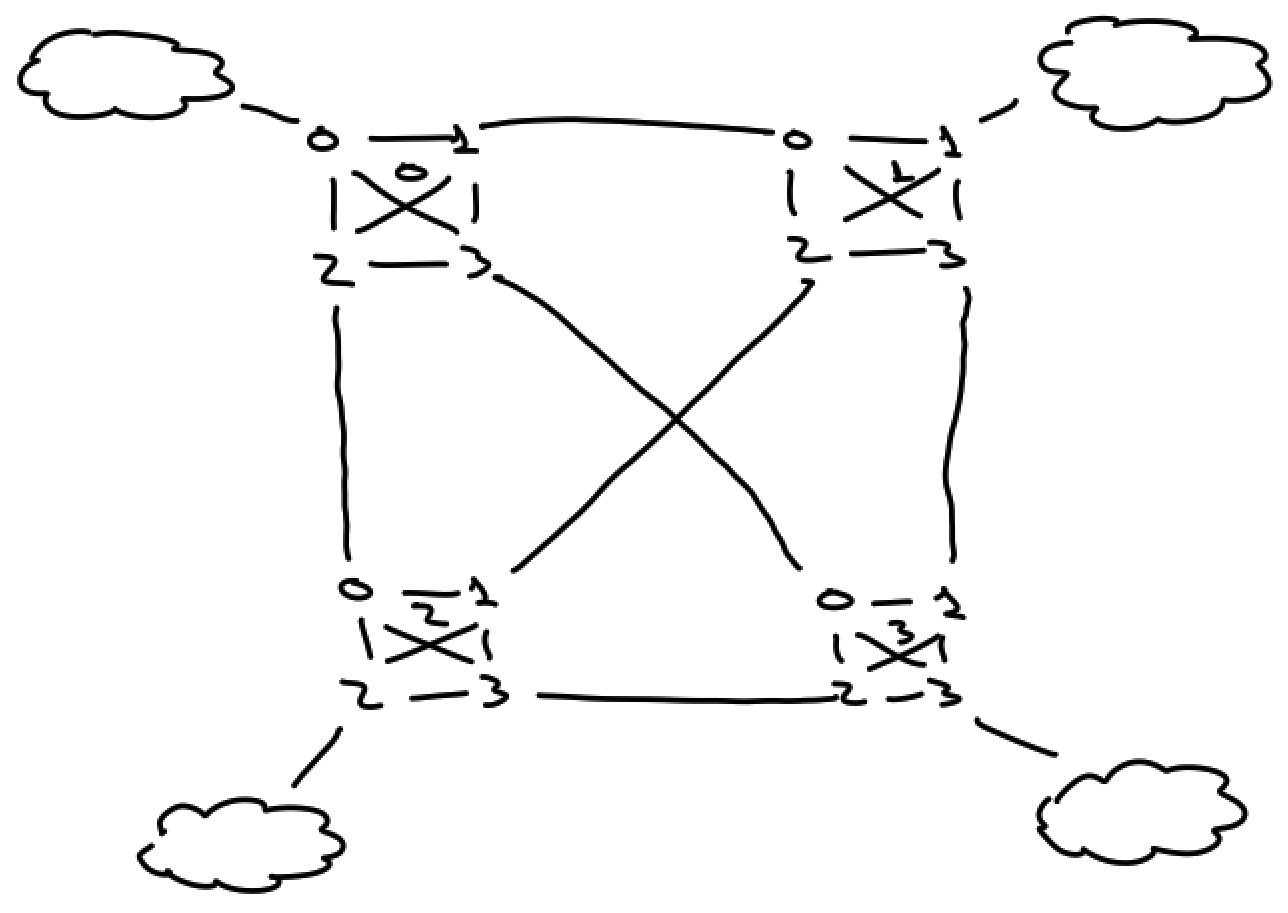
\includegraphics[width=\linewidth]{figures/no-canonica-internet.png}
        \caption{\label{fig:no-canonica-internet} Conexión a internet en la alternativa no canónica}
    \end{subfigure}
    \begin{subfigure}{0.49\textwidth}
        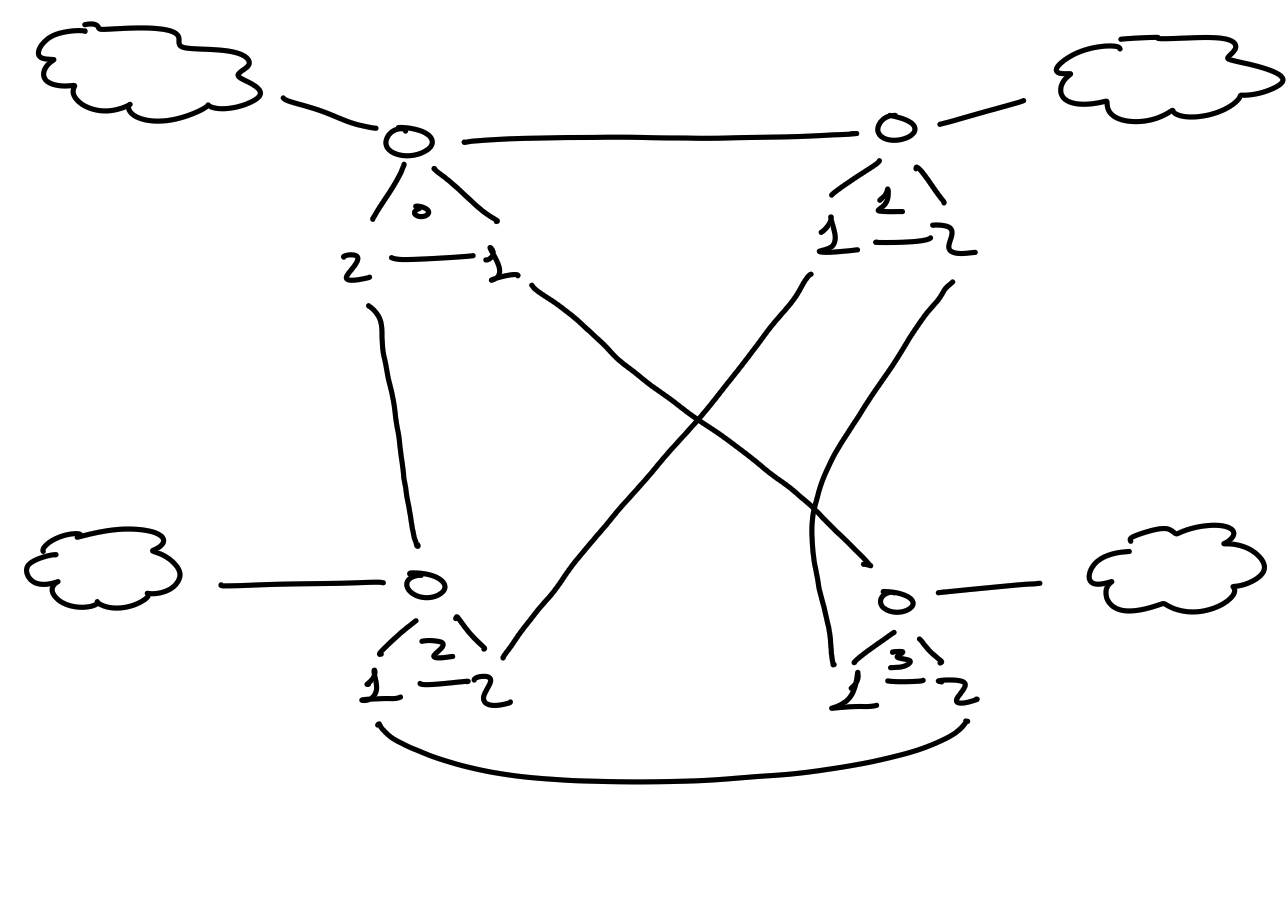
\includegraphics[width=\linewidth]{figures/canonica-internet.png}
        \caption{\label{fig:canonica-internet} Conexión a internet en la alternativa canónica}
    \end{subfigure}
    \caption{\label{fig:conexion-internet} Comparación simplificada de la conexión a internet}
\end{figure}


\chapter{Análisis de Resultados}
\label{ch:análisis-resultados}

\section{Fiabilidad}
\label{sec:fiabilidad}

La fiabilidad de la red es un aspecto crítico en cualquier sistema interconectado, ya que mide la capacidad del sistema para mantenerse operativo incluso en caso de fallos en algunos de sus componentes.

En este diseño, el objetivo de fiabilidad establecido es alcanzar un mínimo del 99.9468556\%, lo que equivale a un nivel muy alto de operatividad y resiliencia frente a fallos. Para calcular la fiabilidad de la red, se ha utilizado la fórmula de la ecuación \ref{eq:prob-fallo-enlaces}, en la cual:

\begin{itemize}
    \item $N$ es el número total de enlaces disponibles en la red
    \item $K$ es el número total de enlaces que fallan simultaneamente
    \item $p$ es la probabilidad de fallo de un enlace individual
\end{itemize}

\begin{equation} \label{eq:prob-fallo-enlaces}
    P[fallo K] = {N \choose K} \cdot p^K \cdot (1 - p)^{N - K}
\end{equation}

Para obtener un cálculo más realista, se han considerado dos escenarios: uno pesimista y otro optimista, los cuales permiten evaluar el rendimiento en situaciones con diferentes niveles de fiabilidad en los enlaces. En ambos escenarios, se ha decidido que $K$ sea igual a 6 enlaces fallidos, lo que representa aproximadamente el 5\% del total de enlaces, un margen razonable para evaluar la robustez del sistema.

\subsection{Escenario Pesimista}
\label{subsec:escenario-pesimista}

En el escenario pesimista, se considera que la probabilidad de fallo de un enlace es relativamente alta. Se ha asumido que la probabilidad de que un enlace falle es de $1 - 0.996079$, lo que indica que cada enlace tiene una pequeña pero significativa posibilidad de fallo.

Al aplicar la fórmula mencionada previamente (ecuación \ref{eq:prob-fallo-enlaces}), se obtiene una fiabilidad global de $99.99915181\%$. Este resultado demuestra que, incluso bajo condiciones pesimistas, la red supera con creces el objetivo mínimo de fiabilidad del $99.9468556\%$. 

Esto es un indicativo positivo, ya que implica que la red es capaz de mantener su funcionamiento casi perfecto incluso en circunstancias adversas, donde hasta el $5\%$ de los enlaces no funcionan.

Cabe destacar que, al cumplir el objetivo de fiabilidad en el escenario pesimista, podría parecer innecesario realizar el cálculo en el escenario optimista. Sin embargo, se llevará a cabo para tener una visión completa del desempeño del sistema bajo diferentes condiciones.

\subsection{Escenario Optimista}
\label{subsec:escenario-optimista}


En el escenario optimista, se asume que los enlaces tienen una probabilidad de fallo mucho menor. En este caso, la probabilidad de fallo de un enlace se ha establecido en $1 - 0.999850$, lo que refleja un sistema de interconexión altamente confiable, donde los fallos son extremadamente raros.

Al introducir esta probabilidad en la fórmula correspondiente (ecuación \ref{eq:prob-fallo-enlaces}), se obtiene un valor de fiabilidad global prácticamente perfecto, alcanzando un impresionante $99.999999999995909843069\%$. 

Este resultado es esencialmente un $100\%$, lo que indica que, en un escenario donde los enlaces fallan muy raramente, la red es capaz de operar sin interrupciones apreciables.

Este escenario optimista confirma que, bajo condiciones ideales, el sistema ofrece una fiabilidad excepcional, garantizando un nivel de servicio casi continuo y asegurando que el impacto de cualquier fallo sea mínimo.

\section{Análisis de Costes}
\label{sec:análisis-costes}

Una vez presentada la arquitectura de la red al completo, junto con sus necesidades de capacidad, se procede a realizar una estimación del coste total. Este coste está dividido en 2 partes: coste de la maquinaria y coste de los enlaces.

\subsection{Coste de la Maquinaria}
\label{subsec:coste-maquinaria}

Para poder realizar una estimación del coste de la maquinaria de la red, hay que hacer un recuento de todos los elementos empleados: $4545$ servidores, $240$ racks y $240$ routers. El precio resultante es:

\begin{itemize}
    \item $4545 \text{ servidores} \cdot 7000 €/\text{servidor} = 31815000 €$
    \item $240 \text{ racks} \cdot 10000 €/\text{rack} = 2400000 €$
    \item $240 \text{ routers} \cdot 6000 €/router = 1440000 €$
\end{itemize}

Total maquinaria = $35655000 €$

\subsection{Coste de los Enlaces}
\label{subsec:coste-enlaces}

Se ha supuesto un tráfico homogéneo a lo largo de toda la red, es decir, que se distribuye uniformemente entre todos los racks. Este enfoque permite simplificar los cálculos y dimensionar la infraestructura más eficientemente. En particular, el tráfico pico a cubrir es de $1.5 \cdot 10^{13}$ bps (15 Tbps). Dado que la red está compuesta por 240 racks, esto se traduce en aproximadamente 62.5 Gbps por rack.

Para asegurar que cada rack tenga capacidad suficiente para manejar este volumen de tráfico, se ha optado por utilizar enlaces de $100$ Gbps. Esta elección responde a dos razones clave:

\begin{enumerate}
    \item Capacidad adicional: Al seleccionar enlaces de 100 Gbps, se garantiza un margen por encima del tráfico homogéneo esperado, lo que proporciona flexibilidad en caso de que el tráfico en algún rack aumente temporalmente. Este enfoque previene cuellos de botella y asegura que los racks puedan manejar cargas más altas sin comprometer el rendimiento general de la red.
    \item Simplicidad en las conexiones: Aunque podría ser más económico utilizar dos enlaces de 50 Gbps en lugar de uno de 100 Gbps, la preferencia por un único enlace responde al deseo de simplificar la infraestructura de red. Al reducir el número de conexiones físicas, se disminuye la complejidad del cableado, se mejora la gestión de la red y se minimizan los puntos de fallo potenciales. Además, la utilización de un solo enlace reduce la necesidad de equilibrar tráfico entre múltiples conexiones, lo que puede complicar el diseño y la operación de la red.
\end{enumerate}

\section{Routing}
\label{sec:routing}

Lo primero que debe considerarse a la hora de diseñar el routing en una red dragonfly es que se trata de una topología que solo alcanza su máximo potencial con algoritmos de routing dinámico. 

Como se ha presentado en la elección de topolgía, una de las ventajas de este tipo de red es la tolerancia a fallos. Existe más de un camino entre dos nodos. El camino más veloz en saltos entre dos nodos de la red siempre es único y tiene exactamente tres saltos asumiendo que la red se ha configurado de forma canónica. Pero sucede a menudo que, a medida que las redes se acercan a la saturación, los caminos con menor número de saltos entre parejas de nodos, son los primeros en saturarse. Por ello mismo, la ventaja de utilizar un algoritmo de routing dinámico es que puede incrementar el throughput de la red dirigiendo el tráfico por caminos alternativos que, a pesar de ser de mayor longitud, están menos concurridos, mejorando la eficiencia de la comunicación y distribuyendo su carga. Además, un sistema de routing estático no para aprovecharía la tolerancia a fallos de la topología.

El uso de un algoritmo de routing dinámico supera el alcance del proyecto actual, que se trata simplemente de una red didáctica. Por esto mismo se va a utilizar routing estático, aunque es importante tener el anterior dato en mente para casos de implementaciones reales.

Se presentan dos maneras diferentes de encargarse del routing estático en la red dragonfly diseñada, diferenciados por el nivel de abstracción de protocolos. Puede hacerse el routing directamente en la capa ethernet mediante switches y direcciones mac (denominado red fabric) o puede subirse una capa más al nivel ip y dirigir el tráfico por routers.

\subsection{Routing a Nivel Ethernet}
\label{subsec:routing-nivel-ethernet}

La primera solución es más eficiente por la necesidad de hardware menos complejo y la reutilización de los switches que ya se encuentran en la propia red. El problema que presenta es a la hora de documentar, automatizar y comprender la distribución de la red en términos de legibilidad.

La solución que se implementa como ejemplo de este tipo de routing se puede ver en la figura \ref{fig:ethernet-routing}.

\begin{figure}
    \centering
    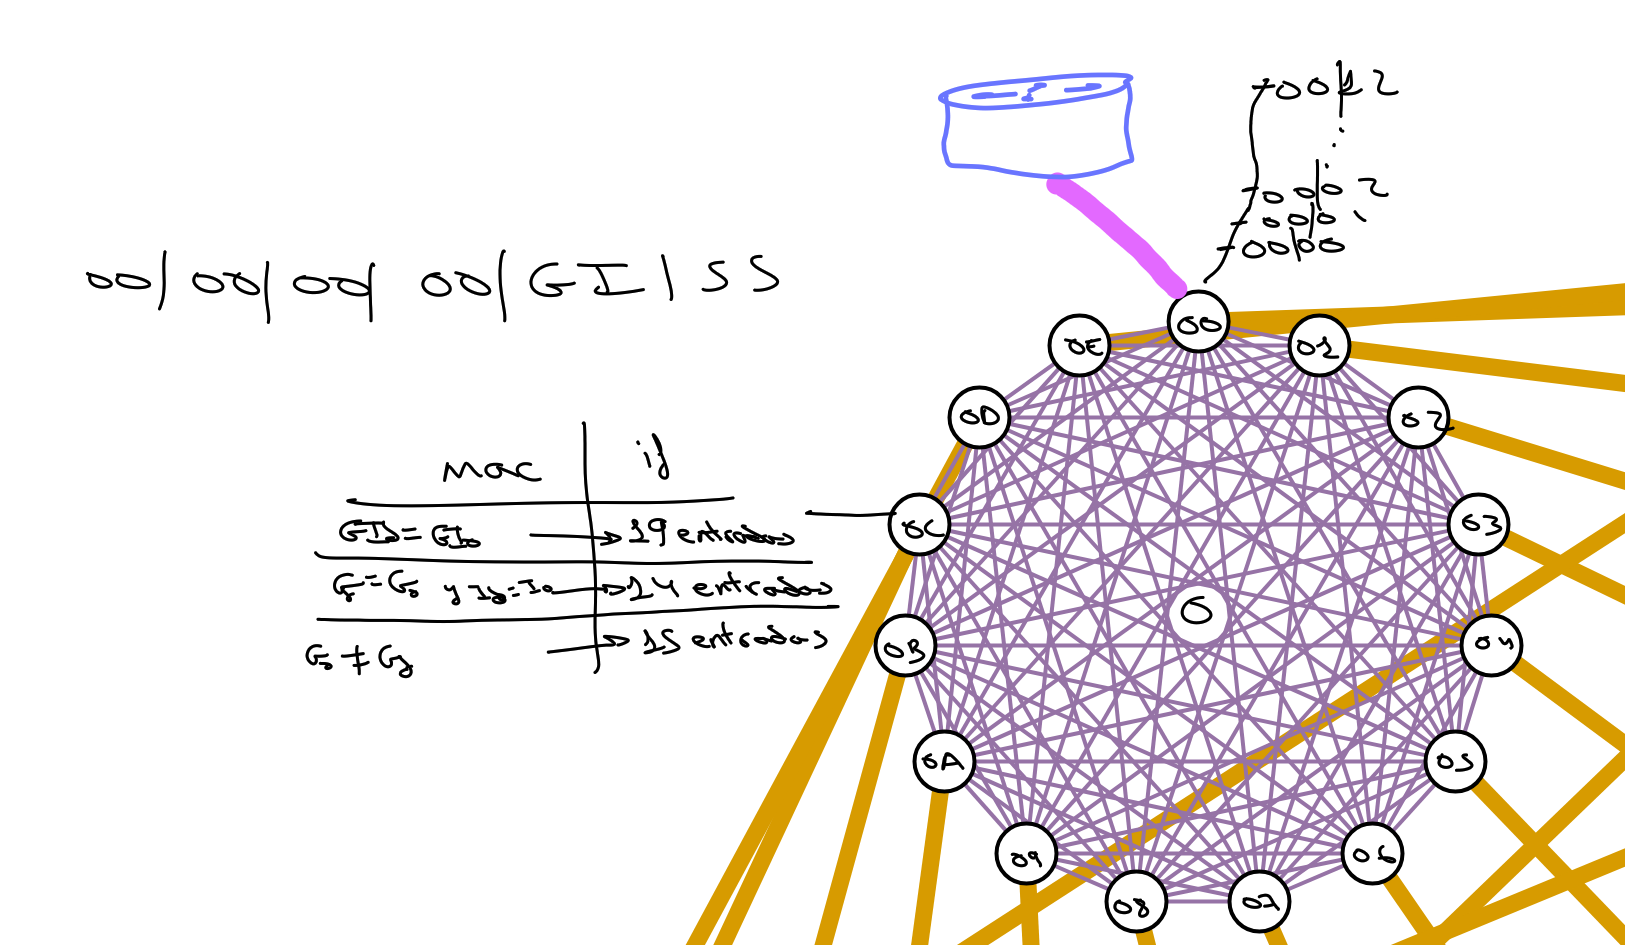
\includegraphics[width=1.0\textwidth]{figures/routing-ethernet.png}
    \caption{\label{fig:ethernet-routing} Configuración de routing a nivel ethernet}
\end{figure}

Cada rack de la red que se presentó en el diagrama anterior (figura \ref{fig:ethernet-routing}) utiliza su switch ''top of the rack'' para dirigir el tráfico entre el resto de racks del grupo y entre los diferentes grupos de la red. Para mejorar la legibilidad se propone alterar las direcciones mac como se muestra en la imagen para que el último byte represente el id del servidor dentro del rack (del 0 al 18 -> cabe dentro de 1 byte (0 a 255)), y el penúltimo byte indique el id del grupo en sus 4 primeros bits y el id del rack dentro del grupo en sus 4 siguientes.

El direccionamiento estático se compone de las siguientes reglas cada una con cierto número de entradas necesarias en la configuración del switch para su debido funcionamiento:

\begin{enumerate}
    \item $GI_d = GI_a$: (19 reglas necesarias) Si el rack destino es el mismo que el del switch actual, una regla  para cada uno de los servidores posibles.
    \item $G_d = G_a$: (14 reglas necesarias) Si el grupo destino es el del switch actual, una regla para cada uno de los racks posibles del grupo menos el actual.
    \item $G_d \neq G_a$: (15 reglas necesarias) Si el grupo destino no es el del switch actual, una regla para cada uno de los switches del grupo, si el camino hacia el grupo destino se alcanza por el switch actual, hacia fuera, si no, hacia el switch que tiene el camino correcto entre grupos.
\end{enumerate}

Siguiendo las reglas anteriores, se configura cada uno de los switches para que se encarguen del routing.

\subsection{Routing a Nivel IP}
\label{subsec:routing-nivel-ip}

Como alternativa al método anterior, define una forma de routing a nivel ip mediante la intervención de routers. Sería necesario un router en cada rack.

El concepto es similar, simplemente a una capa superior de abstracción y por tanto, más sencillo de configurar y mantener. Se puede ver con claridad en la figura \ref{fig:ip-routing}.

\begin{figure}
    \centering
    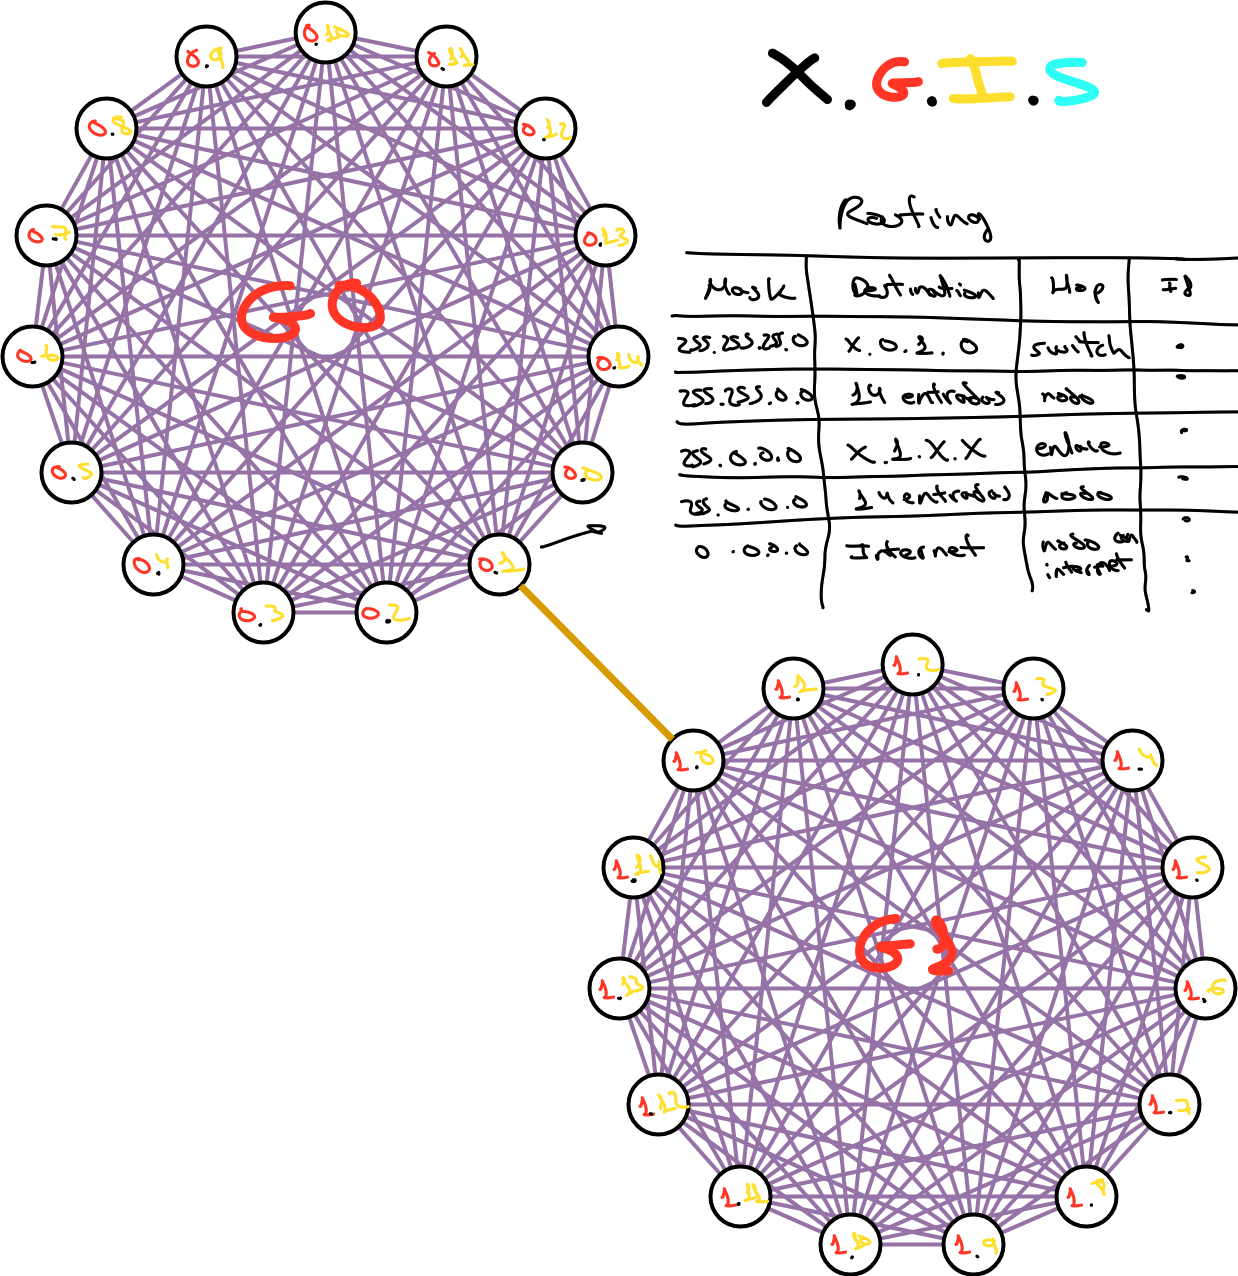
\includegraphics[width=1.0\textwidth]{figures/routing-ip.png}
    \caption{\label{fig:ip-routing} Configuración de routing a nivel ip}
\end{figure}

Como puede verse, en esta solución, las direcciones siguen un patrón similar. Se utiliza el segundo byte para representar el grupo, el tercero para el id de nodo dentro del grupo y el cuarto para el id de servidor dentro del rack. Cada dirección identifica de manera única a cada uno de los servidores de la red.

El routing en esta alternativa se basa en routing ip y sigue las mismas reglas que la solución por switches pero con direcciones ip. La manifestación de estas reglas en la tabla de direccionamiento es obviamente diferente. En la imagen puede verse el ejemplo de tabla de routing ip para el router del nodo 0.1 (grupo 0 rack 1).

\chapter{Conclusiones}
\label{ch:conclusiones}



\chapter{Introducción}
\label{ch:introduccion}

La introducción a un \gls{pfg} o a un \gls{pfm} es el punto de entrada a
todo el trabajo realizado y es considerada la más importante tras el
resumen, donde se resume el trabajo entero. Aquí hay que dejar claro
\textbf{qué} trabajo se ha realizado y el \textbf{porqué} de su
importancia. Se deben generar expectativas. Un gancho típico en los
trabajos suele ser el de aportar un dato relevante o controvertido para
discutir sobre él o plantear una pregunta relevante para el contexto en
el que se está trabajando.

Dentro del capítulo, tras introducir el trabajo realizado, se suelen
incluir las siguientes secciones para establecer bien su alcance y
limitaciones: \textbf{motivación}, \textbf{objetivos},
\textbf{suposiciones/limitaciones} y, a veces,
\textbf{estructura de la memoria}. Ni que decir tiene que esta
estructura planteada, tanto del capítulo como de la memoria en si es
únicamente un ejemplo o propuesta. Cada proyecto es único y a veces es
más cómodo escribirlo de otro modo.

\section{Objetivos}

Es \textbf{la finalidad} del proyecto, y suele encajar en una de las
siguientes categorías:

\begin{itemize}
    \item \textbf{Contraste} o validación de una hipótesis, común en
        \glspl{pfm}.
    \item \textbf{Desarrollo} o diseño de algo (software, hardware,
        sistemas, edificios), común en ingenierías.
    \item \textbf{Estudio} de un tema que deduce o descubre nuevo
        conocimiento, típico en ciencias puras y humanidades.
\end{itemize}

Es muy útil para evaluar el éxito del proyecto, ya que en las
conclusiones se puede determinar qué objetivos se han logrado y cuáles
no, y por qué. Para determinar si un objetivo se ha cumplido, debe ser:

\begin{itemize}
    \item Acotado en el tiempo: Permite establecer un marco temporal y
        planificar.
    \item Medible: Facilita evaluar el progreso hacia un resultado
        aceptable.
    \item Específico: Bien definido para evitar tareas irrelevantes.
    \item Alcanzable: Realista para asegurar su finalización.
    \item Relevante: Debe estar relacionado con el campo de estudio del
        proyecto.
\end{itemize}

Regla mnemotécnica: \gls{amear}.

\section{Motivación}
\label{s:motivacion}

Se refiere a los factores que han hecho que el estudiante se decante por
trabajar en éste tema.

No se trata de decir lo mucho que queríamos trabajar en este tema, o que
es algo que nos ha apasionado desde niños, o que \enquote{queremos
ampliar nuestros conocimientos}. Es más bien buscar la motivación en el
impacto que este trabajo puede tener en nuestro entorno (medioambiental,
social, tecnológico, \ldots).

Algunas fuentes donde encontrar este tipo de motivaciones pueden ser las
revistas especializadas, periódicos, organismos de estandarización,
\glspl{ong}, etcétera.

\section{Justificación}

Esta sección, aunque no es obligatoria, puede ser interesante. Aquí es
donde se explican las razones por las que se eligió este tema, así como
su importancia y relevancia. A veces se junta con la sección anterior
\nameref{s:motivacion}.

Algunos elementos clave que se pueden abordar en esta sección son:

\begin{enumerate}
    \item \textbf{Relevancia del tema}: ¿Existe alguna necesidad o
        problema específico que tu proyecto pueda abordar?
    \item \textbf{Justificación teórica}: Mención sobre qué teorías,
        enfoques o modelos existentes en la literatura respalden la
        importancia de abordar este tema.
    \item \textbf{Brecha en el conocimiento}: ¿Qué aspectos no se han
        explorado lo suficiente o no han sido abordados en estudios
        previos? ¿Cómo puede el proyecto contribuir a cerrar esa brecha
        en el conocimiento?
    \item \textbf{Contribución práctica}: Aplicaciones del proyecto y
        cómo pueden beneficiar a la comunidad académica, profesional o
        a la sociedad en general.
\end{enumerate}

Si se escribe, debe ser lo suficientemente clara y convincente para que
los lectores comprendan por qué el proyecto es relevante y necesario.

\section{Estructura de la memoria}

Esta sección permite al lector comprender la secuencia lógica de cómo se
ha desarrollado el proyecto o la investigación. Presentará un resumen de
los diferentes capítulos que conforman la memoria (a poder ser en un
único párrafo, como mucho dos).

\chapter{¿Cómo estructurar la memoria?}
\label{s:como-estructurar}

Un \gls{pfg} tiene como propósito demostrar que se poseen las destrezas
y los conocimientos que se esperan de un egresado de la titulación
cursada. Esto quiere decir que, a diferencia de otros tipos de trabajo
académico, en éste no es necesario realizar aportaciones originales al
estado de la cuestión sobre el que se trabaja.

¿Y sobre la estructura? \enquote{Como buenamente se quiera/pueda}.
Dependerá del tipode trabajo, pero con carácter general, los trabajos
suelen seguir cierta estructura. La típica suele ser la siguiente:

\begin{enumerate}
    \item Una \textbf{portada} que muestre lo requerido por la normativa
        de la escuela.
    \item Un \textbf{resumen} y un \textbf{\textit{abstract}} resumiendo
        toda la memoria (el primero en español, el segundo en inglés).
    \item Índice de contenidos, de figuras y de tablas, que apuntan a
        los diferentes elementos de interés de la memoria.
    \item La \textbf{introducción}, que explica qué se va a hacer y por
        qué.
    \item El \textbf{estado de la cuestión}\footnote{Se suele decir
        \enquote{estado del arte}, pero se desaconseja su uso por ser
        un anglicismo derivado de la expresión \textit{state of the art}
        en favor expresiones como \enquote{estado de la cuestión}, cosa
        que, por otro lado, suena bastante bien. Más información en
        \url{https://www.rae.es/dpd/arte}.}, donde se dice qué es lo que
        existe sobre lo que se sustenta nuestro proyecto.
    \item La \textbf{metodología} que describe paso por paso el proceso
        de cómo se ha realizado el proyecto.
    \item Los \textbf{resultados} obtenidos tras finalizar el proyecto
        junto con una \textbf{discusión} (en el mismo capítulo o en uno
        nuevo) donde se explican las implicaciones que el autor de la
        memoria considere oportuno destacar sobre los mismos.
    \item Las \textbf{conclusiones} del proyecto, donde el autor indica
        el nivel de consecución de los objetivos, se tira a la piscina
        a la hora de dar respuestas a cuestiones relacionadas con los
        resultados, propone trabajos futuros \textbf{de interés o
        utilidad} (no chorradas) y poco más.
    \item Un apéndice describiendo el impacto social y medioambiental
        del proyecto.
    \item Más apéndices que el autor considere necesarios.
    \item Referencias bibliográficas.
    \item Glosario, abreviaturas y demás.
\end{enumerate}

La plantilla genera automáticamente la portada de acuerdo a los que
dicta la normativa de la escuela, los índices de contenidos, figuras y
tablas, las referencias bibliográficas y los apéndices (con ayuda, por
supuesto, pero se dedicen del marcado). El resto lo tiene que poner el
autor; aun así no te preocupes que es más fácil de lo que parece.

\chapter{Escribiendo la memoria}

¿Cómo comenzamos a escribir la memoria? Con cuidado, y por el principio.
Y el principio es el fichero \texttt{report.tex}, por lo que vamos a ver
las primeras líneasPor el principio, y con cuidado. Esto es, con el fichero \texttt{report.tex}. Veamos la primera línea del fichero (listado~\ref{lst:starting-report}).

\lstinputlisting[
    language=tex,
    firstline=1,
    lastline=5,
    caption=Primeras líneas del fichero \texttt{report.tex},label=lst:starting-report
]{report.tex}

Estos valores configuran gran parte de cómo se comportará el renderizado
de la plantilla. Los parámetros y sus opciones son los siguientes:

\begin{itemize}
    \item \textbf{\texttt{school}}: La escuela a la que pertenece el
        estudiante. Determinará, entre otras cosas, direcciones, formato
        de portada y colores principales. Las opciones se describen en
        el~\autoref{ch:escuelas-y-titulos}.
    \item \textbf{\texttt{type}}: El tipo de memoria. Modifica algunos textos, incluida la portada. Puede tomar los valores \texttt{pfg} (\acrlong{pfg}) y \texttt{pfm}  (\acrlong{pfm}).
    \item \textbf{\texttt{degree}}: El código del grado. Al igual que
    con las escuelas, lo scódigos de los grados soportados se encuentran
    en el~\autoref{ch:escuelas-y-titulos}.
\end{itemize}

Las siguientes líneas (listado~\ref{lst:title-author-and-director})
representan el título del proyecto, el autor o autores más sus entradas
bibliográficas, y el director o directores más sus entradas
bibliográficas.

\lstinputlisting[
    language=tex,
    firstline=10,
    lastline=14,
    caption={Configurando autor, título del proyecto y director},
    label={lst:title-author-and-director}
]{report.tex}

Eso de las entradas bibliográficas para autores y directores no son más
que los nombres que queremos que aparezcan en la segunda página, donde
se indica cómo citar el proyecto. El día que quien está escribiendo esto
aprenda cómo hacerlo automáticamente, este párrafo desaparecerá como
lágrimas en la lluvia\footnote{Bueno, y si tú, queridísima lectora o
lector, si sabes cómo hacerlo, haz un \textit{pull request} al
repositorio de la plantilla: \url{\templaterepository}.}.

\section{Primeros pasos}

Ahora empieza el primer contenido de verdad: el \textbf{resumen} y el
\textbf{\textit{abstract}}. Ambos dos son obligatorios y se añaden con
la macro \lstinline{\abstract}, donde se especificarán el idioma
(\texttt{spanish} o \texttt{english}) y el contenido. En el
\autoref{lst:abstract} se muestran las primeras líneas donde se declara
el resumen de este documento.

\lstinputlisting[
    language=tex,
    firstline=19,
    lastline=22,
    caption={Declarando el resumen en español},
    label={lst:abstract}
]{report.tex}

De la misma forma, las palabras clave se añaden con la macro
\lstinline{\keywords}. Son obligatorios, así que no te los saltes.

\lstinputlisting[
    language=tex,
    firstline=38,
    lastline=44,
    caption={La lista de palabras clave en español},
    label={lst:keywords}
]{report.tex}

También existe la opción de añadir agradecimientos con
\lstinline{\acknowledgements}. Si no se pone no se muestra en el
documento final, pero es algo bonito y a las abuelas les encanta
aparecer ahí. Y las abuelas son de lo más bonito que existe en este
mundo, así que cuidadlas.

\section{Empezando con la memoria en sí}

Y ahora sí, empezamos con la memoria del proyecto en si. Habrá que ir
escribiendo un capítulo tras otro. En este ejemplo está todo escrito en
el mismo fichero (\texttt{report.tex}), pero es muy común escribirlo en
varios ficheros diferentes e ir incluyéndolos mediante la macro
\lstinline{\include}, tal y como se muestra en el~\autoref{lst:include}.

\begin{lstlisting}[
    language=tex,
    caption=Incluyendo ficheros externos en el documento,
    label=lst:include]
\include{introduction.tex}
\include{state-of-the-art.tex}
\include{methodology.tex}
\include{results.tex}
\include{conclusions.tex}
\end{lstlisting}

Una vez hemos terminado de escribir los capítulos principales, la macro
\lstinline{\appendix} indica desde qué punto empiezan los apéndices. No
son obligatorios, ni mucho menos, pero en algunos \glspl{pfg} y
\glspl{pfm} los incluyen para dar información adicional que no se
considera clave en el contenido de la memoria, pero que es interesante
para complementarla. Por ejemplo, en un \gls{pfm} para el estudio del
comportamiento de conductores al volante, uno de los apéndices podría
ser cada uno de los formularios que se le ofrecieron para rellenar a
cada uno de los conductores de dicho estudio.

Y ya estaría todo. Resumiendo, hay que configurar la plantilla, poner
el autor, título y director del proyecto e incluir los capítulos y
apéndices que queramos.

\section{El caso concreto de los PFM}

Un \gls{pfm}, a diferencia de un \gls{pfg} trata de profundizar más en
un campo concreto de una disciplina, por lo que tiene a ser más extenso
y mucho más específico.

En términos generales, la estructura es similar. Sin embargo es de
esperar que el nivel de exigencia sea mayor, ya que el estudiante que
lo realiza debe demostrar que es un titulado superior. Esto se nota más
en la fase de documentación, ya que al tratar de profundizar en un tema
más específico, el trabajo de contextualizar y argumentar es más
tedioso.

Se pueden identificar dos tipos de proyectos diferentes, aquellos que
podríamos catalogar de \textit{profesionales}, con enfoque a la
innovación o mejora en un área profesional concreta, y aquellos
\textit{de investigación}, más enfocados a la búsqueda de nuevo
conocimiento en el área, y que suelen ser el comienzo de la carrera
investigadora.

\section{Reglas y recomendaciones}

TODO: Explicar el el PFG es trabajo del estudiante, el profesor realiza la supervisión. Es trabajo autónomo del alumno y debe llegar a un resultado.

TODO: Prevenir contra el uso de IA generativa al tuntún


\chapter{Componentes de la plantilla}
\label{ch:componentes-de-la-plantilla}

En este capítulo hablaremos de los componentes principales con los que trabajaremos en nuestra memoria.

\section{Columnas}

TBD

\section{Ecuaciones}

La facilidad de composición de ecuaciones es una de las cosas que más atrae de \LaTeX\space a muchos autores. \LaTeX mantiene dos renderizadores diferentes, uno para el texto y otro para las ecuaciones, denominados modo párrafo y modo matemático\footnote{Existe un tercer modo, denominado \textit{LR mode} o \textit{left-to-right mode}, raramente utilizado y que no trataremos aquí}. El modo párrafo es el modo por defecto y no se le llama explícitamente. Al modo matemático, sin embargo, se le invoca de varias maneras diferentes.

\subsection{Modo en párrafo}

La forma más común es la forma ``en línea'', donde el texto para el modo matemático se encierra entre dos signos \$. Por ejemplo, veamos la frase del listado~\ref{lst:in-line-equation}.

\begin{lstlisting}[language=tex,caption=Ejemplo de inserción de fórmulas en linea,label=lst:in-line-equation]
El pequeño teorema de Fermat dice que si $p$ es un número primo, entonces, para cada número natural $a$, con $a>0$, $a^p \equiv a (\mod p)$
\end{lstlisting}

La frase quedaría como sigue:

El pequeño teorema de Fermat dice que si $p$ es un número primo, entonces, para cada número natural $a$, con $a>0$, $a^p \equiv a (mod p)$

\subsection{Ecuaciones en bloque}

Cuando en lugar de poner una ecuación dentro de un párrafo existente la queremos insertar en su propio espacio independiente hacemos uso de los entorno \texttt{equation} o \texttt{align}, dependiendo de si queremos una o más ecuaciones en el bloque, respectivamente. Por ejemplo, en el caso de una única ecuación, sería similar al ejemplo siguiente:

\begin{minipage}[c]{.5\textwidth}
\begin{lstlisting}[language=tex]
\begin{equation}
	\int_a^b f'(x) \, dx=f(b)-f(a)
\end{equation}
\end{lstlisting}
\end{minipage}%
\begin{minipage}[c]{.5\textwidth}
\begin{equation}
    \int_a^b f'(x) \, dx=f(b)-f(a)
\end{equation}
\end{minipage}

Sin embargo, en el caso de que quisiésemos más de una ecuación en el mismo bloque haríamos uso del carácter \& para indicar en qué punto se alinean las ecuaciones; por ejemplo:

\begin{minipage}[c]{.5\textwidth}
\begin{lstlisting}[language=tex]
\begin{align}
    u  &= \arctan x \\ 
    du &= \frac{1}{1 + x^2}dx
\end{align}
\end{lstlisting}
\end{minipage}%
\begin{minipage}[c]{.5\textwidth}
\begin{align}
    u  &= \arctan x \\ 
    du &= \frac{1}{1 + x^2}dx
\end{align}
\end{minipage}

Por último, si no tenemos por qué referenciarlas en el texto, podemos hacer uso de los entornos \texttt{equation*} y \texttt{align*}.

\begin{minipage}[c]{.5\textwidth}
\begin{lstlisting}[language=tex]
\begin{equation*}
    \int_a^b f'(x) \, dx=f(b)-f(a)
\end{equation*}
\end{lstlisting}
\end{minipage}%
\begin{minipage}[c]{.5\textwidth}
\begin{equation*}
    \int_a^b f'(x) \, dx=f(b)-f(a)
\end{equation*}
\end{minipage}

En caso de querer generar un índice de ecuaciones del documento, de la misma manera que los listados de Figuras, Tablas y Listados. Para ello, debemos añadir a la lista de ecuaciones la ecuación definida con el comando \texttt{myequations}. Es importante destacar que para generar un listado de ecuaciones estas deben estar numeradas, es decir.

\begin{minipage}[c]{.5\textwidth}
\begin{lstlisting}[language=tex]
\begin{equation}
     \frac{x^2}{a^2} - \frac{y^2}{b^2} = 1
\end{equation}
\myequations{Ecuación canónica de la hipérbola}
\end{lstlisting}
\end{minipage}%
\begin{minipage}[c]{.5\textwidth}
\begin{equation}
     \frac{x^2}{a^2} - \frac{y^2}{b^2} = 1
\end{equation}
\end{minipage} 

\section{Elementos flotantes}

Vamos a hablar un poco de los elementos denominados \enquote{flotantes} o \textit{floats}. Éstos son bloques de contenido que \enquote{flotan} por la página hasta que \hologo{LaTeX} los coloca donde considera a través de ciertos algoritmos.

Lo general es \textbf{declarar el elemento flotante inmediatamente después del párrafo donde se ha referenciado} (las referencias cruzadas las vemos en la~\autoref{s:crossref} de este capítulo), y después dejar que \LaTeX\space elija el mejor sitio. Y si después de haber escrito todo el documento hay algo que no cuadre, pues ahí modificarlo.

\enquote{¿Y si no hago referencia a un elemento flotante, dónde lo pongo?} Bueno, pues en general no se pone. Si algo no es nombrado, suele ser porque no aporta información, y si no la aporta, pues para qué lo vamos a meter. Ojo, que lo mismo existe algún caso donde sí tiene sentido, pero es muy raro.

Aunque más adelante veremos los diferentes tipos de \textit{floats}, en caso de que queramos modificar su comportamiento todos tienen los especificadores de posición indicados en la tabla~\ref{tab:floats-options}:

\begin{table}
    \caption{\label{tab:floats-options}Opciones para los elementos flotantes de \hologo{LaTeX}}
    \centering
    \begin{tabularx}{\textwidth}{@{}lX@{}}
        \toprule
        \textbf{Especificador} & \textbf{Acción} \\
        \midrule
        H & Colocar exactamente en el sitio indicado                       \\
        h & Colocar aproximadamente en el sitio indicado                   \\
        t & Colocar al comienzo de la página                               \\
        b & Colocar al final de la página                                  \\
        p & Colocar en una página exclusiva para elementos ``flotantes''   \\
        ! & Forzar las opciones obviando los mecanismos internos de \LaTeX \\
    \bottomrule
    \end{tabularx}
\end{table}

\subsection{Código fuente}

Para la gestión de los listados de código fuente se utiliza el paquete \texttt{listings}. El estilo usado es una modificación\footnote{En realidad la modificación es cambiar el fondo de crema a blanco} de \href{https://ethanschoonover.com/solarized/}{Solarized} desarrollado por Ethan Schoonover.

Existen muchas formas diferentes de incluir listados de código en una memoria. Aquí introducimos los más comunes.

\subsubsection{Código dentro del propio párrafo}

TBD

\subsubsection{Bloques de código}

Insertar código en párrafos no es tan común como insertar bloques enteros. Para ello haremos uso del entorno \texttt{lstlisting}. Por ejemplo:

\lstinputlisting[language=tex, firstline=1, lastline=6]{sources/adding-blocks.tex}

Nos daría el siguiente resultado:

\lstinputlisting[language=python, firstline=2, lastline=5]{sources/adding-blocks.tex}

Una cosa que hay que tener en cuenta es que dentro de un entorno \texttt{lstlisting} se ignoran todos los comandos de \LaTeX\space\footnote{En realidad no todos, y si no mira en estos fuentes cómo hemos metido el fin de bloque \texttt{lstlisting} dentro del propio bloque.} y el texto se imprime tal y como se ha introducido. Esto incluye los tabuladores y espacios de principio de línea.

Al igual que en el código de párrafo, también podemos especificar en qué lenguaje está escrito el código para que se resalten en éste las palabras reservadas. Por ejemplo:

\lstinputlisting[language=tex, firstline=8, lastline=14]{sources/adding-blocks.tex}

Nos daría como resultado el siguiente bloque de código:
 
\lstinputlisting[language=python, firstline=9, lastline=12]{sources/adding-blocks.tex}

\subsubsection{Código directamente desde fichero}

Esta forma es muy común, ya que se usa tanto para hacer referencia al código fuente de la aplicación directamente, como a código separado en ficheros para mantener el tamaño de la memoria manejable.

Suponiendo que tenemos el fichero \texttt{sources/snippets.py}, para incluirlo entero basta con usar el comando \texttt{lstinputlisting}:

\begin{lstlisting}[language=TeX]
\lstinputlisting[language=python]{sources/snippets.py}
\end{lstlisting}

Con este comando conseguiríamos el siguiente resultado:

\lstinputlisting[language=python]{sources/snippets.py}

En caso de que se desease importar sólo parte del fichero, se pueden indicar las filas que delimitan el trozo de código. Por ejemplo:

\begin{lstlisting}[language=TeX]
\lstinputlisting[
    language=python,
    firstline=4,
    lastline=5
]{sources/snippets.py}
\end{lstlisting}

Esto haría que sólo se imprimiesen las filas 4 y 5, correspondientes a la segunda función:

\lstinputlisting[language=python, firstline=4, lastline=5]{sources/snippets.py}

Ambas opciones son opcionales, y los valores por defecto de \texttt{firstline} y \texttt{lastline} serán el principio y el final del fichero respctivamente.

\subsubsection{Etiquetando bloques de código}

Al igual que con el resto de bloques \textit{float} (e.g. figuras o tablas), se pueden\footnote{Pongo \textit{pueden} porque es opcional, pero en realidad se \textbf{deben} poner, porque si no los listados de fuentes quedan horribles, como el de esta plantilla por ejemplo (échale un vistazo si no lo has hecho antes).} (\textbf{deben}) añadir pies de texto a los bloques de código, lo cual hace más legible su cometido.

Para ello basta con añadir el argumento \texttt{caption} a las opciones del bloque. Por ejemplo:

\lstinputlisting[language=tex, firstline=15, lastline=20]{sources/adding-blocks.tex}

Nos daría como resultado el siguiente bloque de código:
 
\lstinputlisting[language=python, firstline=16, lastline=19, caption=Función para determinar cuando una palabra \texttt{w1} es anagrama de otra palabra \texttt{w2}]{sources/adding-blocks.tex}

\subsection{Figuras}
\label{ch:figuras}

El código siguiente (listado~\ref{lst:figure-basic-insert}) renderizará una imagen.

\begin{lstlisting}[language=python, caption=Inserción de una figura,label={lst:figure-basic-insert}]
\begin{figure}
    \centering
    
\includegraphics[width=0.25\textwidth]{figures/vault-boy.png}
    \caption{\label{fig:img-vault-boy} Vault Boy approves that}
\end{figure}
\end{lstlisting}

La sintaxis es bastante autoexplicativa. El entorno \texttt{figure} es el que delimita el contenido de la figura. El comando \texttt{centering} determina que se tiene que centrar . Luego, el comando \texttt{caption} determina el pie de imagen, el cual además incluye una etiqueta (comando \texttt{label}) que sirve para referenciar. Por último, se incluye la imagen con el comando \texttt{includegraphics}.

En definitiva, la imagen (figura~\ref{fig:img-vault-boy}) se mostrará con un ancho igual al 25\% del ancho que ocupa el texto, centrada, con un pie de foto y una etiqueta para referenciar.

\begin{figure}
    \centering
    
\includegraphics[width=0.25\textwidth]{figures/vault-boy.png}
    \caption{\label{fig:img-vault-boy} Vault Boy approves that}
\end{figure}

El comando \texttt{includegraphics} puede importar los formatos típicos de imagen, como jpeg, png o pdf. También admite una serie de opciones como rotación, alto, ancho (éste le hemos especificado con \texttt{width}), etcétera. ¡Ojo! Siempre que se pueda, hay que intentar insertar imágenes vectoriales. De esta manera, se mantiene la calidad de la imagen. Si no, puede ocurrir que se pixele y no quede nada bien.

\subsubsection{Subfiguras}

¿Y qué pasa cuando queremos incluir múltiples imágenes dentro de una figura? Bueno, pues aquí hay que usar el entorno \texttt{subfigure}. En el listado~\ref{lst:subfigure-basic-insert} vemos un ejemplo de cómo se manejan.

\begin{lstlisting}[language=python, caption=Inserción de varias subfiguras,label={lst:subfigure-basic-insert}]
\begin{figure}
	\centering
	\begin{subfigure}{.3\textwidth}
		
\includegraphics[width=\linewidth]{figures/vault-boy.png}
		\caption{\label{fig:subfigure-1}Vault Boy 1}
	\end{subfigure}%
	\begin{subfigure}{.3\textwidth}
		
\includegraphics[width=\textwidth]{figures/vault-boy.png}
		\caption{Vault Boy 2}
	\end{subfigure}%
	\begin{subfigure}{.3\textwidth}
		
\includegraphics[width=\textwidth]{figures/vault-boy.png}
		\caption{Vault Boy 3}
	\end{subfigure}
	\caption{\label{fig:subfigures}Todos los Vault Boy}
\end{figure}
\end{lstlisting}

En realidad cada subfigura se trata como una figura normal, pero en relación con el \textit{float} contenedor. Cuando a una subfigura se le especifica un ancho, se le está diciendo al compilador de qué ancho es esa subfigura en concreto (en nuestro caso 0.3 veces el ancho de la línea). Sin embargo, a la imagen se le da un ancho total de \texttt{linewidth}, porque al estar dentro de su espacio de subfigura, el ancho ha cambiado. El resultado es el que se observa en la figura~\ref{fig:subfigures}. Por cierto, también podemos referenciar a los pies de las subfiguras (e.g. Así:~\ref{fig:subfigure-1}).

\begin{figure}
	\centering
	\begin{subfigure}{.3\textwidth}
		
\includegraphics[width=\linewidth]{figures/vault-boy.png}
		\caption{\label{fig:subfigure-1}Vault Boy 1}
	\end{subfigure}
    \hfill
	\begin{subfigure}{.3\textwidth}
		
\includegraphics[width=\textwidth]{figures/vault-boy.png}
		\caption{Vault Boy 2}
	\end{subfigure}
    \hfill
	\begin{subfigure}{.3\textwidth}
		
\includegraphics[width=\textwidth]{figures/vault-boy.png}
		\caption{Vault Boy 3}
	\end{subfigure}
	\caption{\label{fig:subfigures}Todos los Vault Boy}
\end{figure}

\subsection{Tablas}

Las tablas (en realidad \enquote{cuadros}, pero bueno) son una forma muy eficaz de presentar información. En los resultados de casi cualquier trabajo existen cuadros de algún tipo para que los datos se comprendan de un único vistazo (o para que al menos sea más fácil identificarlos.

Sin embargo, las tablas suelen ser bastante complicadas en \LaTeX, por lo menos para la gente que empieza. Para no escribir demasiado, la respuesta para casi toda maquetación de tabla está en \href{https://www.tablesgenerator.com/}{https://www.tablesgenerator.com/}. En serio, no perdáis el tiempo si no es estrictamente necesario. La maquetáis visualmente, la generáis (con estilo \textit{booktabs}) y a correr.

\section{Enlaces de hipertexto}

TBD

\section{Fórmulas matemáticas}

TBD

\section{Glosario}
\label{s:glosario}

El glosario de una memoria es el lugar donde se encuentran los términos que se usan a lo largo del documento y que se considera que requieren una aclaración. En esta plantilla, en el momento que generemos un término, se creará un capítulo al final de la memoria con el listado de todos aquellos términos definidos.

Para gestionar el glosario se hace uso del paquete \texttt{glossaries} el cual es relativamente complejo de configurar. También su documentación es muy extensa\footnote{Pero aún así es el sitio donde ir a buscar información. El paquete, junto con su documentación está disponible en la dirección \href{https://www.ctan.org/pkg/glossaries}{https://www.ctan.org/pkg/glossaries}.}, así que en esta sección hablaremos únicamente de lo esencial.

\subsection{¿Cuándo y cómo especificar términos?}

La regla general del \enquote{cuándo} es una vez terminada la memoria. En ese punto, seremos conscientes de qué términos son los más interesantes para incluir en el glosario. En ese punto deberemos ir término por termino sustituyéndolo por la entrada del glosario para que el proceso automático se encargue de la indexación y numeración de páginas.

El \enquote{cómo} se refiere a de qué manera escribirlos. La regla general en el castellano (y hasta donde el autor de la plantilla sabe, en cualquier idioma) es de la manera en la que aparecería en medio del texto. Es decir, si la palabra se escribe generalmente en minúscula (e.g.~\textit{El jugador blandía un \gls{hacha-batalla}}) se deberá incluir dentro del glosario en minúscula, mientras que si se escribe generalmente en mayúscula (e.g.~\textit{Encontró el \gls{arco-perdicion}}) irá en mayúscula.

\subsection{Definiendo los términos del glosario}

Las entradas se escribirán dentro del fichero \texttt{frontmatter/glossary.tex}. La forma estándar de definir un término es la que se muestra en el listado~\ref{lst:std-glossary-entry}.

\begin{lstlisting}[language={[latex]TeX},caption=Código para crear una entrada en el glosario,label=lst:std-glossary-entry]
\newglossaryentry{hacha-batalla}{
    name={hacha de batalla},
    description={Herramienta antigua utilizada en combate}
}
\end{lstlisting}

Luego, dentro del texto, podremos hacer referencia a dichas entradas con los comandos que se muestran en la tabla~\ref{tab:glossary-commands}.

\begin{table}
    \caption{\label{tab:glossary-commands}Comandos para incluir términos del glosario en el texto de la memoria}
    \begin{tabularx}{\textwidth}{@{}lX@{}}
        \toprule
        \textbf{Comando} & \textbf{Ejemplo con la clave \texttt{hacha-batalla}} \\
        \midrule
        \texttt{\textbackslash gls} & \gls{hacha-batalla} \\
        \texttt{\textbackslash Gls} & \Gls{hacha-batalla} \\
        \texttt{\textbackslash glspl} & \glspl{hacha-batalla} \\
        \texttt{\textbackslash Glslp} & \Glspl{hacha-batalla} \\
        \bottomrule
    \end{tabularx}
\end{table}

Como los plurales los gestiona automáticamente, puede ser que queramos, como en este caso, modificar el plural de nuestro término. Para ello debemos añadir la opción \texttt{plural} a la entrada para especificar cómo es el plural de la entrada, como se muestra en el listado~\ref{lst:gls-longplural}.

\begin{lstlisting}[language={[latex]TeX},caption=Especificando el plural para un término del glosario,label=lst:gls-longplural]
\newglossaryentry{python}{
    name={Python},
    plural={Pythonacos},
    description={El mejor lenguaje de programación}
}
\end{lstlisting}

Así, el plural de la clave \texttt{python} descrita quedaría como \glspl{python}, en lugar del valor por defecto que sería \textit{Pythons}.

Un caso particular de términos del glosario son las siglas y los acrónimos. No vamos a entrar en detalle aquí\footnote{Pero recomendamos visitar \href{https://www.fundeu.es/recomendacion/siglas-y-acronimos-claves-de-redaccion/}{https://www.fundeu.es/recomendacion/siglas-y-acronimos-claves-de-redaccion/} y darle una leída porque es interesante.} sino que vamos a introducir las siglas como caso especial de entrada de glosario. Cuando tengamos una sigla, la crearemos en el glosario como se muestra en el listado~\ref{lst:new-acronym}.

\begin{lstlisting}[language={[latex]TeX},caption=Entrada genérica de una sigla o acrónimo en el glosario,label=lst:new-acronym]
\newacronym[
    description={Proyecto Fin de Grado. Proyecto a realizar al final de una titulación de Grado},
    longplural={Proyectos Fin de Grado}
    ]{pfg}{PFG}{Proyecto Fin de Grado}
\end{lstlisting}

En el ejemplo se puede ver que hay dos entradas, \texttt{longplural} y \texttt{description} que son opcionales. La primera es la equivalente a \texttt{plural} de \texttt{newglossaryentry}, y no necesita más explicación.

La segunda, \texttt{description} suele utilizarse para acrónimos, cuando necesitamos describir la entrada. Cuidado en este caso porque si hace referencia a varias palabras estas se deberían incluir dentro de la descripción (como en el ejemplo, \enquote{\acrlong{pfg}}).

La regla general de los acrónimos y las siglas es que la primera vez que aparecen en el texto, deben aparecer con el nombre completo mientras que el resto de veces pueden aparecer indistintamente como sigla o forma larga. De esto se encarga automáticamente el comando \texttt{gls}. Es decir, si tenemos la sigla \texttt{special}, la primera vez que incluyamos la sigla con \texttt{\textbackslash gls\{special\}} saldrá \gls{special} mientras que el resto de veces que la incluyamos se verá simplemente \gls{special}.

Con los acrónimos se incluyen comandos adicionales para controlar su presentación. Estos son los mostrados en la tabla~\ref{tab:acronym-commands}

\begin{table}
    \caption{\label{tab:acronym-commands}Comandos específicos para controlar la presentación de acrónimos}
    \begin{tabularx}{\textwidth}{@{}lX@{}}
        \toprule
        \textbf{Comando} & \textbf{Ejemplo con la clave \texttt{rpg}} \\
        \midrule
        \texttt{\textbackslash acrshort} & \acrshort{rpg} \\
        \texttt{\textbackslash acrshortpl} & \acrshortpl{rpg} \\
        \texttt{\textbackslash acrlong} & \acrlong{rpg} \\
        \texttt{\textbackslash Acrlong} & \Acrlong{rpg} \\
        \texttt{\textbackslash acrlongpl} & \acrlongpl{rpg} \\
        \texttt{\textbackslash Acrlongpl} & \Acrlongpl{rpg} \\
        \texttt{\textbackslash acrfull} & \acrfull{rpg} \\
        \texttt{\textbackslash Acrfull} & \Acrfull{rpg} \\
        \texttt{\textbackslash acrfullpl} & \acrfullpl{rpg} \\
        \texttt{\textbackslash Acrfullpl} & \Acrfullpl{rpg} \\
        \bottomrule
    \end{tabularx}
\end{table}

Por cierto, en castellano las siglas \textbf{no incluyen la \enquote{s} al final}, así que no deberíamos usar los comandos que terminan en \texttt{pl}. Por eso la definición que se ha hecho de la sigla \texttt{rpg} es la mostrada en la figura~\ref{fig:acronym-rpg}.

\begin{lstlisting}[language={[latex]TeX},caption=Entrada de \texttt{rpg} en \texttt{glossaries.tex},label=fig:acronym-rpg]
\newacronym[
    description={Role-Playing Game. Juego de rol},
    shortplural={RPG}
    ]{rpg}{RPG}{\textit{Role-Playing Game}}
\end{lstlisting}

\section{Notas}

TBD

\section{Referencias cruzadas}
\label{s:crossref}

Las etiquetas (\textit{label}) son una herramienta muy útil en el proceso de composición tipográfica. Se puede pensar en ellas como punteros a zonas de interés del documento, de tal manera que se les pueda referenciar sin necesidad de conocer su posición final en la composición.

Por ejemplo, lo normal es que en un libro, a la hora de referenciar una figura, aparezca una frase del estilo ``[\ldots] como muestra la Figura 3 [\ldots]''. Lo que es bastante raro son las frases del estilo ``[\ldots] como muestra la Figura de los moñecos amarillos [\ldots]'' o ``[\ldots] como muestra la siguiente Figura [\ldots]''\footnote{Sí, bueno, quizá la segunda frase no es tan rara, pero siempre es preferible referenciar directamente a dar posiciones relativas.}.

Una de las propiedades más útiles y, en ocasiones, infravaloradas de \LaTeX es la facilidad y potencia de su sistema de etiquetado. Este sistema permite referenciar tablas, listados de código fuente, ecuaciones, capítulos, secciones, etc., con facilidad y flexibilidad. Además, \LaTeX las numera y referencia automáticamente, cambiando la numeración en función de las adiciones y supresiones sin que el autor tenga que hacer nada.

Para referenciar un elemento, lo primero que hay que crear es una etiqueta \textbf{después} del elemento a referenciar. Esto ya lo hemos visto anteriormente, por ejemplo en el listado~\ref{lst:figure-basic-insert}. Si nos fijamos, se declara una etiqueta justo después de la etiqueta \texttt{caption} con el nombre \texttt{fig:img-vault-boy}. De esta manera, podemos referenciar varios indicadores de la figura, como se muestra en el listado~\ref{lst:basic-references}

\begin{lstlisting}[language=tex, caption=Referenciando una figura y su página,label={lst:basic-references},]
Mira la Figura~\ref{fig:img-vault-boy} en la página~\nameref{fig:img-vault-boy}.
\end{lstlisting}

Dicho listado daría el siguiente resultado:

\blockquote{Mira la Figura~\ref{fig:img-vault-boy} titulada \nameref{fig:img-vault-boy} en la página~\pageref{fig:img-vault-boy}.}

\notebox{
    \textbf{¿Por qué a mí me aparece el símbolo \texttt{??} en lugar de una referencia?} Pues lo más seguro es que sea un error a la hora de escribir la etiqueta. Menos común, pero también puede pasar, es que el documento no se haya compilado bien. Hay que tener en cuenta que \LaTeX\space fue creado en una época donde las máquinas tenían poca (¡poquísima!) RAM, y para funcionar lo que se hacían eran varias compilaciones sobre el documento, almacenando los valores temporales en ficheros. Y como nadie quiere perder tiempo en cambiar y \textit{debuggear} algo que funciona estupendamente bien, no se reimplementa. De todas formas, si te animas, ahí tienes un buen proyecto que si lo sacas adelante te va a hacer muy famoso.
}

\section{Referencias bibliográficas}
\label{s:referencias-bibliograficas}

Hay muchas formas diferentes hacerlo, así que en esta plantilla hemos
decidido elegir una de ellas por considerarla la más cómoda y simple,
que es mediante el paquete \textit{biblatex}.

El fichero de referencias \texttt{references.bib}, incluirá una entrada
por cada una de las referencias que se citan (o no) durante la memoria.
Luego, en el cuerpo del texto, se podrán hacer referencias a estas. Será
\LaTeX~después quien se encargue de indexar correctamente, crear los
hipervínculos y maquetar automáticamente.

Las referencias que no aparezcan citadas en el texto no aparecerán en el
capítulo de referencias, cosa que tiene sentido porque si no se habla de
ellas, ¿para qué las vamos a nombrar?

\notebox{
    \textbf{No has dicho en ningún momento \textit{bibliografía}} Ya.
    Las referencias bibliográficas, también conocidas como lista de
    referencias o simplemente referencias, son todas aquellas fuentes
    bibliográficas que han sido citadas a lo largo del documento. La
    bibliografía, también conocida como referencias externas, es
    simplemente una lista de recursos utilizados, citados o no. Como
    generalmente los no referenciados no se usan para dar soporte a un
    texto científico se suelen descartar.
}

\subsection{¿Cómo creamos nuevas referencias?}

El fichero \texttt{references.bib} contará cero o más entradas con la estructura mostrada en el listado~\ref{lst:base-bibref}.

\begin{lstlisting}[language=tex,caption=Estructura general de una referencia,label=lst:base-bibref]
@tipo{id,
    author = "Autor",
    title = "Título de la referencia (libro, artículo, enlace, ...)",
    campo1 = "valor",
    campo2 = "valor",
    \ldots
}
\end{lstlisting}

En esta entrada, \texttt{@tipo} indica el tipo de elemento (p. ej.
\texttt{@article} para artículos o \texttt{@book} para libros) e
\texttt{id} es un identificador \textbf{único en todo el documento} para
el elemento. El resto de campos dependerán del tipo de la referencia,
aunque generalmente casi todos los tipos comparten los campos de
\texttt{author}, \texttt{title} o \texttt{year}.

\subsection{¿De qué manera puedo citar las referencias?}

Pues básicamente hay dos estilos: sin paréntesis, donde el autor y el
año aparecen para dar un estilo narrativo, y con paréntesis, donde
aparecen entre paréntesis, dando a entender que no forman parte de la
narrativa. Se usan tal y como se muestra en el listado~\ref{lst:bibref}.

\begin{lstlisting}[
    language=tex,
    caption=Referenciando una entrada bibliográfica,
    label={lst:bibref},
    ]
Tal y como describen \cite{mcculloch1943logical}, las neuronas
artificiales son la caña \parencite{mcculloch1943logical}.
\end{lstlisting}

Algo que queda como sigue:

\enquote{Tal y como se describen \cite{mcculloch1943logical}, las
neuronas artificiales son la caña \parencite{mcculloch1943logical}.}

\subsection{Más información}

Tienes muchas más información acerca de las referencias bibliográficas
en \href{https://bibtex.eu/es/biblatex/}{\hologo{BibTeX}.eu}\footnote{
Url: \url{https://bibtex.eu/es/biblatex/}. Último acceso el 18 de julio
de 2024.}.

\section{Referencias cruzadas}

TBD

\section{Referencias a recursos externos}

TBD

\chapter{Licencia}
\label{ch:licencia}

Cuando se publica la obra en el archivo digital, por defecto lo hace con la licencia de \textit{Creative Commons} Reconocimiento - Sin obra derivada - No comercial. Aunque usar esta licencia es correcto, no es una licencia libre y a algunos nos parece algo malo.

Considero que todo el conocimiento generado en una universidad pública ha de ser público y libre. Por ello esta obra se publica con la licencia \textit{Creative Commons} Reconocimiento - Sin obra derivada - No comercial - Compartir igual, de tal manera que se garantiza que la obra se comparte con las mismas libertades y así, todo el mundo puede hacer de esta obra el uso que quiera.

\appendix

\chapter{¿Cómo ampliar la plantilla?}
\label{ch:ampliar}

TBD

\chapter{Escuelas y títulos}
\label{ch:escuelas-y-titulos}

A continuación se describen todas las opciones de grados y títulos disponibles en la memoria.

\section{Escuelas}

Las escuelas disponibles se describen en el cuadro~\ref{tbl:schools}.

\begin{table}
    \centering
    \begin{tabularx}{\textwidth}{@{}lX@{}}
        \toprule
        \textbf{Clave}   & \textbf{Valor} \\
        \midrule
        \texttt{etsiaab} & E.T.S. de Ingeniería Agronómica, Alimentaria y de Biosistemas \\
        \texttt{etsidi}  & E.T.S. de Ingeniería y Diseño Industrial \\
        \texttt{etsisi}  & E.T.S. de Ingeniería de Sistemas Informáticos \\
        \bottomrule
    \end{tabularx}
    \caption{\label{tbl:schools} Relación entre el código de la plantilla y la escuela a la que se refiere}
\end{table}

De momento no están todas, así que si te apetece añadir la tuya puedes, o bien contactar con los autores, o bien modificarlo (mira el apéndice~\ref{ch:ampliar}) y también contactar con los autores, así lo podemos hacer público con la mayor cantidad de usuarios posible.

\section{Titulaciones}

Cada una de las escuelas poseen ciertas titulaciones que se han de añadir a la configuración.

\subsection{E.T.S. de Ingeniería Agronómica, Alimentaria y de Biosistemas}

La ETSIAAB tiene configurados como colores principal y de link el RGB $(99,178,76)$.

Las titulaciones que existen la última vez que se actualizó este documento son las siguientes:

\begin{itemize}
    \item \texttt{20BT}: Grado en Biotecnología,
    \item \texttt{20BI}: Grado en Ciencias Agrarias y Bioeconomía,
    \item \texttt{20IG}: Grado en Ingeniería Agrícola,
    \item \texttt{02IA}: Grado en Ingeniería Agroambiental,
    \item \texttt{20IA}: Grado en Ingeniería Alimentaria.
\end{itemize}

\subsection{E.T.S. de Ingeniería y Diseño Industrial}

La ETSIDI tiene configurados como colores principal y de link el RGB $(223,30,64)$.

Las titulaciones que existen la última vez que se actualizó este documento son las siguientes:

\begin{itemize}
    \item \texttt{56IE}: Grado en Ingeniería Eléctrica,
    \item \texttt{56IA}: Grado en Ingeniería Electrónica Industrial y Automática,
    \item \texttt{56IM}: Grado en Ingeniería Mecánica,
    \item \texttt{56IQ}: Grado en Grado en Ingeniería Química,
    \item \texttt{56DD}: Grado en Ingeniería en Diseño Industrial y Desarrollo de Producto.
\end{itemize}

\subsection{E.T.S. de Ingeniería de Sistemas Informáticos}

La ETSISI tiene configurados como colores principal y de link el RGB $(0,114,206)$.

Las titulaciones que existen la última vez que se actualizó este documento son las siguientes:

\begin{itemize}
    \item \texttt{61CD}: Grado en Ciencia de Datos e Inteligencia Artificial,
    \item \texttt{61CI}: Grado en Ingeniería de Computadores,
    \item \texttt{61IW}: Grado en Ingeniería del Software,
    \item \texttt{61SI}: Grado en Sistemas de Información,
    \item \texttt{61TI}: Grado en Tecnologías para la Sociedad de la Información.
\end{itemize}


\end{document}
